%! Author = Saeid Yazdani
%! Date = 7/22/2024


\section{The Feedback Signal Resolution}
\label{sec:feedback-signal-resolution}

According to \autoref{fig:ringing-in-multistage-loops}, the input to the control
path is multiplied by the product of all gain blocks, therefore the output
can be calculated by \autoref{eq:output-voltage}.

\begin{equation}
    \label{eq:output-voltage}
    V_{OUT} = {G_1}{G_2}{G_3}{V_{in}}
\end{equation}

Be $G_1$ a typical op-amp with a gain of $400,000$ and $G_2=35$ to
get \SI{\pm350}{\volt} out of a \SI{\pm10}{\volt} control swing
and $G_3=1$ (since it is being used as a current booster with unity gain, as
explained later in \autoref{subsec:current-booster-considerations}) we
will get a gain product of $14,000,000$.

Having a DAC with N bit, and an \ac{FSR} of 1 to 10V, we get the
quantization step values ($V_{in}=V_{out}/G_{total}$):

\begin{table}[h]
    \centering
    \begin{tabular}{cc}
        \toprule
        \textbf{Output Voltage} & \textbf{Input Voltage Difference} \\
        \midrule
        \SI{1}{\volt}           & \SI{70}{\nano\volt}               \\
        \SI{10}{\volt}          & \SI{700}{\nano\volt}              \\
        \SI{100}{\volt}         & \SI{7}{\micro\volt}               \\
        \SI{350}{\volt}         & \SI{25}{\micro\volt}              \\
        \bottomrule
    \end{tabular}
    \caption{Voltage Output and Differential Input}
    \label{tab:output-vs-input-differentials}
\end{table}

According to \autoref{tab:resolutions-requirements-list}, only a \ac{DAC} with
$\ge$24-bit meets the requirements; however, we need to use a multiplying DAC
with variable reference input voltages to achieve the desired quantization.
If a fixed \ac{FSR} is used, a 26-bit to 28-bit DAC will be necessary to attain
the minimum quantization.

\begin{table}[h]
    \centering
    \begin{tabular}{lS[table-format=3.1]S[table-format=3.1]S[table-format=3.1]S[table-format=3.1]}
        \toprule
        \textbf{Resolution} & \textbf{FSR \SI{1}{\volt}} & \textbf{FSR \SI{2.5}{\volt}} & \textbf{FSR \SI{5}{\volt}} &
        \textbf{FSR \SI{10}{\volt}} \\
        \midrule
        16 bit & \SI{15}{\micro\volt}   & \SI{38}{\micro\volt}  & \SI{76}{\micro\volt}  & \SI{152}{\micro\volt} \\
        18 bit & \SI{3.8}{\micro\volt}  & \SI{10}{\micro\volt}  & \SI{19}{\micro\volt}  & \SI{38}{\micro\volt}  \\
        20 bit & \SI{1}{\micro\volt}    & \SI{2.4}{\micro\volt} & \SI{5}{\micro\volt}   & \SI{9.5}{\micro\volt} \\
        22 bit & \SI{0.24}{\micro\volt} & \SI{0.6}{\micro\volt} & \SI{1.2}{\micro\volt} & \SI{2.4}{\micro\volt} \\
        24 bit & \SI{60}{\nano\volt}    & \SI{150}{\nano\volt}  & \SI{300}{\nano\volt}  & \SI{600}{\nano\volt}  \\
        26 bit & \SI{15}{\nano\volt}    & \SI{37}{\nano\volt}   & \SI{75}{\nano\volt}   & \SI{150}{\nano\volt}  \\
        28 bit & \SI{4}{\nano\volt}     & \SI{9}{\nano\volt}    & \SI{19}{\nano\volt}   & \SI{37}{\nano\volt}   \\
        \bottomrule
    \end{tabular}
    \caption{Resolution and \ac{FSR} Voltages}
    \label{tab:resolutions-requirements-list}
\end{table}


The system resolution requirements listed above necessitate the use of
\emph{Sub-Ranging} converters which involve using multiple stages
(\emph{coarse} and \emph{vernier}\footnote{Also known as \emph{fine} or
\emph{residual} stage.}) to achieve high-resolution
and accurate analog output that would otherwise not be possible with
single-stage DACs due to their limited number of output bits and lack of
precision.
The concept of sub-ranging DACs and the calculation of the final output are 
given in
\autoref{fig:subranging-concept} and \autoref{eq:subranging-summation}
respectively:

\begin{figure}[h]
    \centering
    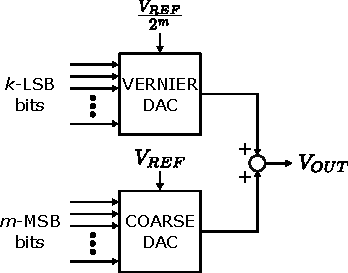
\includegraphics[width=0.64\linewidth,height=0.37\textheight,keepaspectratio]
    {figures/dps_algorithms_psu/subranging-concept}
    \caption[Sub-Ranging \acs{DAC}s Concept]{
        Sub-ranging concept by combining two \acp{DAC}.
        The \emph{coarse} \acs{DAC} is responsible for setting the approximate
        value of the desired output while
        the \emph{vernier} \acs{DAC} adjusts the output of the coarse \acs{DAC}
        with higher precision.
        It usually has higher resolution but covers a smaller range and
        fine-tunes the output by adding or subtracting a small value to the
        signal produced by the coarse \acs{DAC}.
    }
    \label{fig:subranging-concept}
\end{figure}

\begin{equation}
    \label{eq:subranging-summation}
    \begin{aligned}
        V_{OUT} = \biggl(&\frac{b_0}{2} + \frac{b_1}{4} + \cdots + \frac{b_{m-1}}{2^m} \\
                         &+ \frac{b_m}{2^{m+1}} + \frac{b_{m+1}}{2^{m+2}} + \cdots
                         + \frac{b_{m+k-1}}{2^{m+k}}\biggr) V_{REF}
    \end{aligned}
\end{equation}

Initially, \emph{coarse} signals are generated, and the residue error is
minimized through the \emph{vernier} stage.
To ensure that resolution and accuracy are matched, error correction is
required, and therefore, sub-ranging converters incorporate transfer curve
correction methods to overcome non-linearity in coarse and vernier stages.

The output word is then calculated by \autoref{eq:output-subranging} as the
result of adding each stage ($S$) and their associated
errors ($E$) and corrections ($C$).
We may assume the error of the vernier stage is zero since it will be
within the noise levels, and therefore the correction can also be skipped.

\begin{equation}
    \label{eq:output-subranging}
    S_{OUT} = {S_{COARSE} + E_{COARSE} + C_{COARSE}} + S_{VERNIER}
\end{equation}

The \ac{MSB} of the vernier converter corresponds to the smallest increment that
can be added by the coarse converter's \ac{LSB}.
Therefore, \ac{MSB} of the vernier stage
must be more precise than \ac{LSB} of the coarse stage.

In addition, the range for correction factors in the coarse stage must be greater than
its maximum error so that the system has the required headroom for the
vernier converter to keep the total output within a defined error bound.
Therefore, the correction factor in the coarse stage must be sufficiently
large to account for the maximum possible error, so that
$ran(C_{COARSE}) > max(E_{COARSE})$.

Whenever the capabilities of the vernier converter are limited
to less than the maximum error of the coarse stage, the system can
face missing codes on the DAC input and distortions in the combined output of
the converters.

\autoref{fig:subranging-signal} shows a detailed view of the converter
signals:

\begin{figure}[htbp]
    \centering
    \printfitgraphics[0.62\textheight]{figures/dps_algorithms_psu/subranging-correction}
    \caption[Sub-Ranging Converter Signal]{
        Comparison of an ideal response and true response of a
        sub-ranging converter where two non-matching codes are encircled.
        If the residual error left by the coarse converter is larger than what
        the vernier converter can accurately represent, vernier converter
        may \emph{saturate} and will not be able to differentiate between
        neighboring values.
	With enough headroom in the vernier converter, reaching word-length
        limit and gross errors can be avoided.
    }
    \label{fig:subranging-signal}
\end{figure}

\begin{enumerate}[topsep=8pt,itemsep=4pt,partopsep=4pt, parsep=4pt]
    \item
    In an ideal world, the coarse converter is precise to the total resolution
    of the combined converter (i.e. one \acs{LSB} of the vernier converter).

    \item
    Precision requires that the \ac{DNL} of the vernier converter be
    $2^{-N_{VERNIER}}$.
    For a 16-bit vernier converter, this means the \acs{DNL} of the coarse
    converter must be less than 0.00001 LSB, which is
    unachievable for higher-resolution converters.
    Therefore, the vernier converter must compensate for all errors in the
    coarse converter without encountering word length limitations.
    This implies that the minimum real-world vernier span must be larger than
    the quantum step of the coarse converter.
    To achieve this, we must know all errors of the coarse converter and a
    description of the coarse transfer curve will be stored in memory.

    \item
    During runtime, we assemble the full target word length ($W$) for ($N$-bit)
    sub-ranging according to \autoref{eq:vernier-word-calculation}.

    \item
    If the vernier converter's word length is not sufficient to represent the
    necessary precision, it won't be able to accurately correct the errors from
    the coarse stage. In that case, the vernier converter cannot
    differentiate between small changes in the residual error.

    \item
    If the vernier converter hits its word length limit, it can no longer
    linearly or smoothly correct errors, causing the transfer curve to have
    abrupt changes or "disruptions."

    \item
    Gross errors can occur when the converter fails to handle the residual
    errors properly.
    These errors can lead to large gaps between the intended and actual output
    of the system, rendering the system unreliable.

\end{enumerate}

\begin{equation}
    \label{eq:vernier-word-calculation}
    \begin{split} % breaks long equation in multi-lines
        W_{TOTAL} = W_{COARSE} + W_{FINE} \times 2^{-N_{COARSE}} +
        \\
        C_{COARSE} \times 2^{-N_{COARSE}}
    \end{split}
\end{equation}
